\documentclass[prl,reprint,showpacs,floatfix,nofootinbib]{revtex4-1}
\usepackage{epsfig,graphics,float,amsmath,mathtools}
\usepackage[colorlinks=true,citecolor=blue]{hyperref}
\usepackage{microtype,setspace,siunitx,physics,epsfig,graphicx}
\usepackage[caption=false]{subfig}
\usepackage{xcolor}
\usepackage[export]{adjustbox}
\usepackage{nameref,physics}
\usepackage{blindtext}
\captionsetup[subfigure]{labelformat=brace}
\usepackage[english]{babel}
%\definecolor{originblue}{RGB}{139,255,167}
%\definecolor{origingreen}{HTML}{fdae61}


\begin{document}
\title{Generating Simulated Data for Machine Learning Training Sets: Particle and Topological Defect Identification and Tracking}

\date{\today}
\author{Adam~A.~S.~Green}
\author{Eric~N.~Minor}
\author{Stian~D.~Howard}
\author{Cheol Park}
\affiliation{Department of Physics and Soft Materials Research Center, University of Colorado, Boulder, Colorado, 80309, USA}


\begin{abstract}
    \blindtext{}
\end{abstract}

\maketitle

\section{Introduction}
%context (ag)
\blindtext{}

\section{Experimental System}

To confirm the veracity of our neural network, a test system is needed for which both reliable simulated data can be generated and physical experimental data captured. Simulations are generated using a variety of methods including Monte Carlo simulations and Landau Gin. In the physical system topological defects are generated on the surface of a Smectic C thin film by quickly changing the pressure gradient across the two sides of the film.

\subsection{Simulation Data}
%\ Need Adam to help with this section

\subsection{Experimental Data}

At the center of our setup is a pressure chamber with an open aperture on the top to draw a film over. When pressure is provided to the chamber through a tube, the film balloons outward. A valve on the tube is then opened to the atmosphere, rapidly venting the pressure to the atmosphere. The valve is controlled by a computer program written to trigger the camera to start recording as well as track the pressure in chamber over time, all of which happens when a defined pressure difference between the chamber and atmosphere is achieved. 

% Confirm 

Smectic C liquid crystal films allow defects to be visualized with partially, or fully, crossed polarizers. In our setup, polarized light is shined perpendicularly onto the film. The reflected light is collected into a microscope where it passes through a partially crossed polarizer. Finally a high speed camera (Phantom V12.1) collects the images at 500 frames per second, and an exposure time of 1900 $\mu$s in gray-scale.

\begin{figure}
  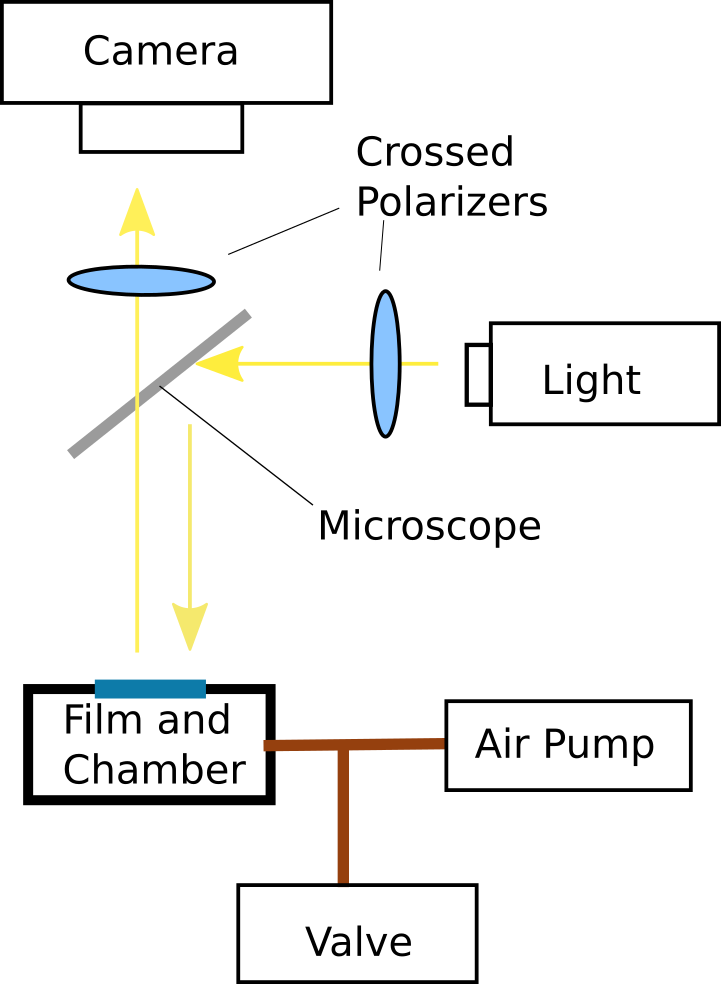
\includegraphics[width=\linewidth]{setup_sketch.png}
  \caption{Sketch of the setup}
  \label{fig:Setup Sketch}
\end{figure}


Each video lasts a little over 12 seconds, capturing the entirety of the short term dynamics. Images are 1104x800  and have a 12 bit pixel grey scale precision, allowing for high contrast to be gained in post processing. When the polarizers are fully crossed, the reflected light is so dim that the images turn out fully black at the exposure time used -- a value which can't be increased due to the frame rate. Partially crossed polarizers allow for more light to reach the camera's CCD while still allowing for visualization of a defect.

\begin{figure}
  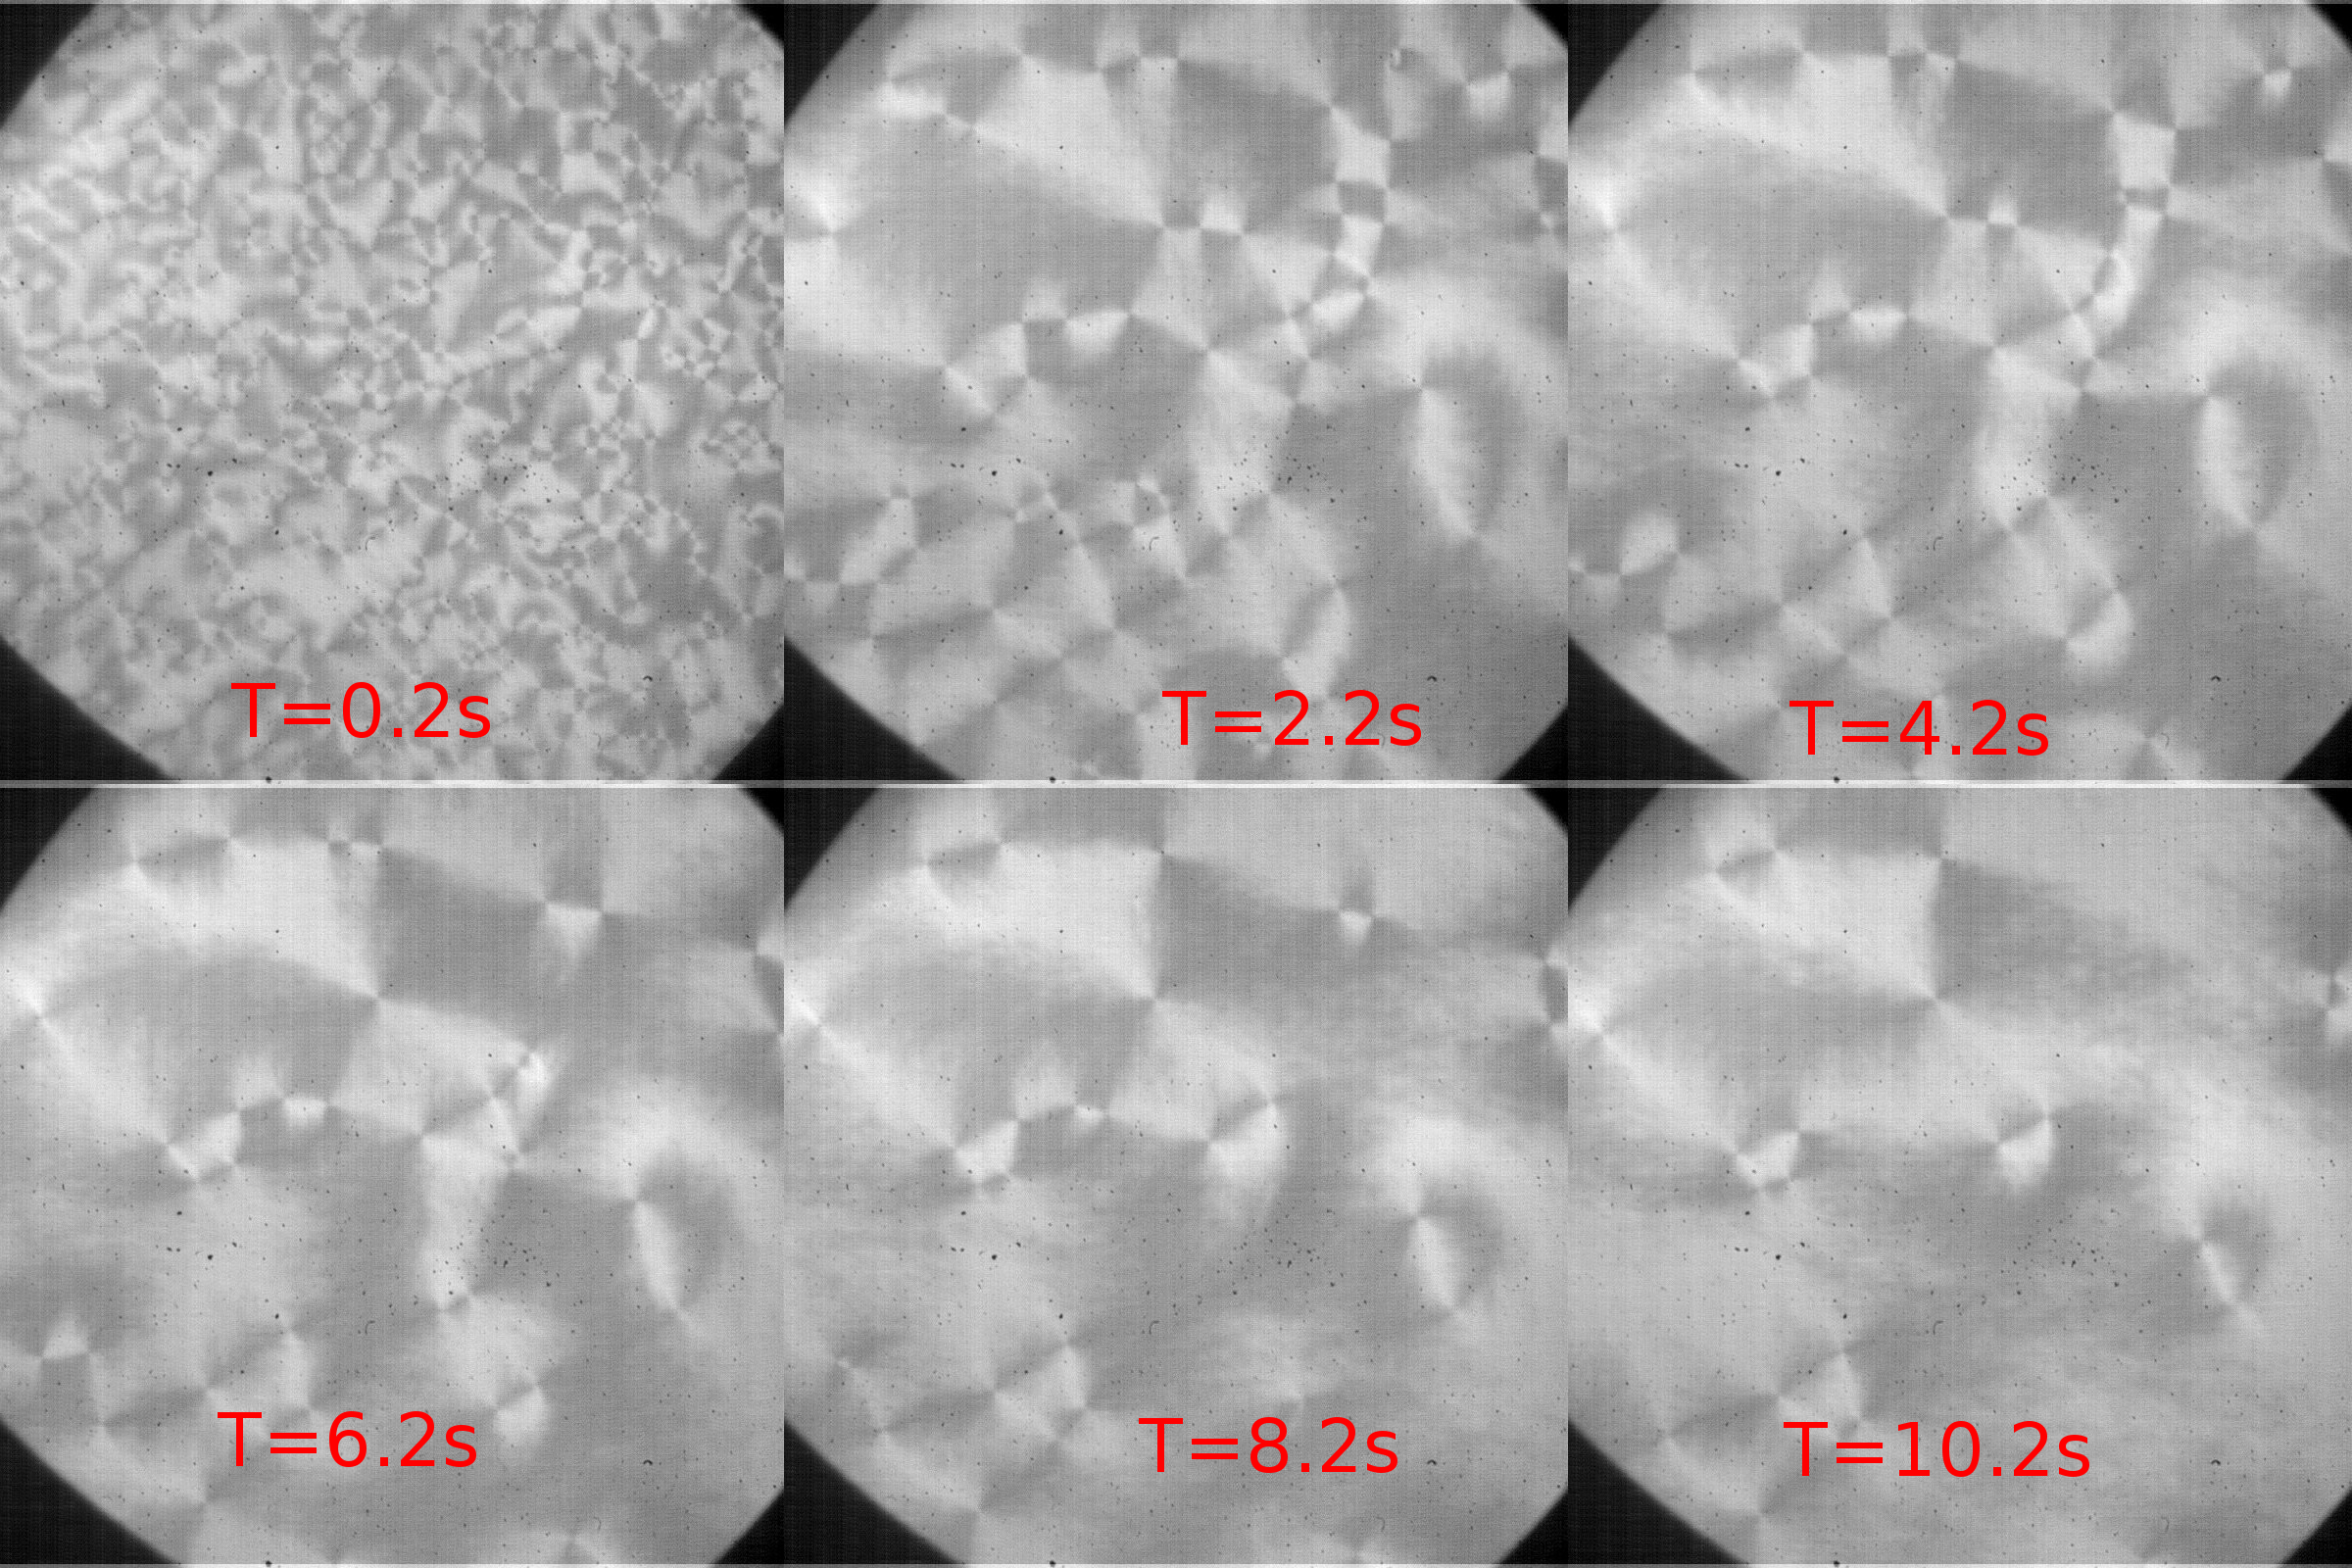
\includegraphics[width=\linewidth]{film.png}
  \caption{Time evolution of a film}
  \label{fig:frames}
\end{figure}

\section{Machine Learning Pipeline}

Previous work has been done demonstrating the viability of using machine learning to identify whether a given simulated photo contains a topological defect [citation]. However, the system was only run on simulated images and did not identify the locations of defects in the images, limiting its usefulness for experimental purposes. In order to make a system viable for usage with real experiments, we developed a pipeline that makes use of modern deep-learning object detection and image enhancement techniques. 

\subsection{Pipeline and Image Enhancement Motivation}

For object detection we used darkflow, which is a TensorFlow implementation of the YOLOv2 algorithm [citation]. YOLOv2 learns to perform both region-proposal and region classification using the darknet-19 architecture. Allowing the region proposal mechanism to be trained is important for our task of defect identification as object detection algorithms that rely on traditional heuristic searches, such as R-CNN [citation], would likely fail to identify the central point of a defect as an object. Training darkflow on a set of 100 simulated 200x200 images with each image containing 20 defects showed that this network is viable for detecting the locations of defects in simulation data. However, the network trained on the pure simulated data was unable to identify defects in experimental images until data enhancement techniques were used to improve the utility of the simulation images.

FIGURE

Machine learning algorithms, by nature, optimize themselves to perform as well as their architecture allows on the given training data. While this can lead to highly effective systems, it is the primary reason why training on a set of simulated data often makes the final model non-viable for usage in the real world. Simulated data is highly predictable and clean while real world data can have large amounts of noise and significant variance in how certain key objects appear. By training on the simulated data, the system will over-fit on the very specific shapes, colors, and gradients produced by the simulation. Since the objects of interest in the experimental data are almost guaranteed to not be as perfect as the ones in the simulation, the machine learning model will fail to identify them. Our solution to this problem is to introduce various inaccuracies, which mimic real-world inaccuracies, into the simulated images, with the goal of making the final model more robust.

\subsection{Standardization and Simulated Image Enhancement}

The first issue that needs to be dealt with is lighting and contrast. In simulated defect images, the intensity of a pixel ranges from perfectly black to perfectly white depending on the director orientation, maximizing the gradients and contrast in the image. The mean intensity of the image will also generally be around 0.5 on a scale from 0 to 1, since there is no offset to the image brightness. When using an experimental image, the difference in brightness between perfectly aligned and perfectly misaligned directors is much smaller than the full dynamic range of the image, causing much smaller gradients. The average brightness of the experimental data is rarely 0.5, so what constitutes bright and dark pixels is more complex than just the intensity of the pixel. To make the simulation and experimental images as similar as possible in regards to average intensity and dynamic range, a common standardization procedure is used. Each pixel's intensity value is set according to the feature standardization formula 

$$ x' = \frac{x - \Bar{x}}{6\sigma} +0.5 $$

where x' is the output pixel intensity, x is the input intensity of each pixel and sigma is the standard deviation of the image pixel intensities. The output pixel intensities now have a mean of 0.5 and a dynamic range of six standard deviations. This procedure reasonably standardizes the lighting and contrast of the images regardless of the actual lighting and camera conditions.

In machine learning, training data is traditionally a hand labelled subset of the larger data-set to be analyzed. We, however, are attempting to train our algorithm with auto annotated simulation data that is more perfect than the experimental data. By adding imperfections to the simulation images, we hope to emulate the experimental data and improve the abilities of the neural network.

Due to the relatively low lighting on the images, the camera read noise, generated by the camera hardware, is significant relative to the signal size. Applying a 2-D discrete Fourier transform, the composition of the image is extracted in the frequency domain (Figure Reference). The high frequencies in the corners contain the information of interest, while the periodic read noise appears as regular lines. Removing the higher frequency spaces, the inverse Fourier transform yields the actual noise pattern of the camera. This characteristic camera noise can then be added as high-frequency noise to the simulated data set to improve veracity to real experimental data.

\begin{figure}
  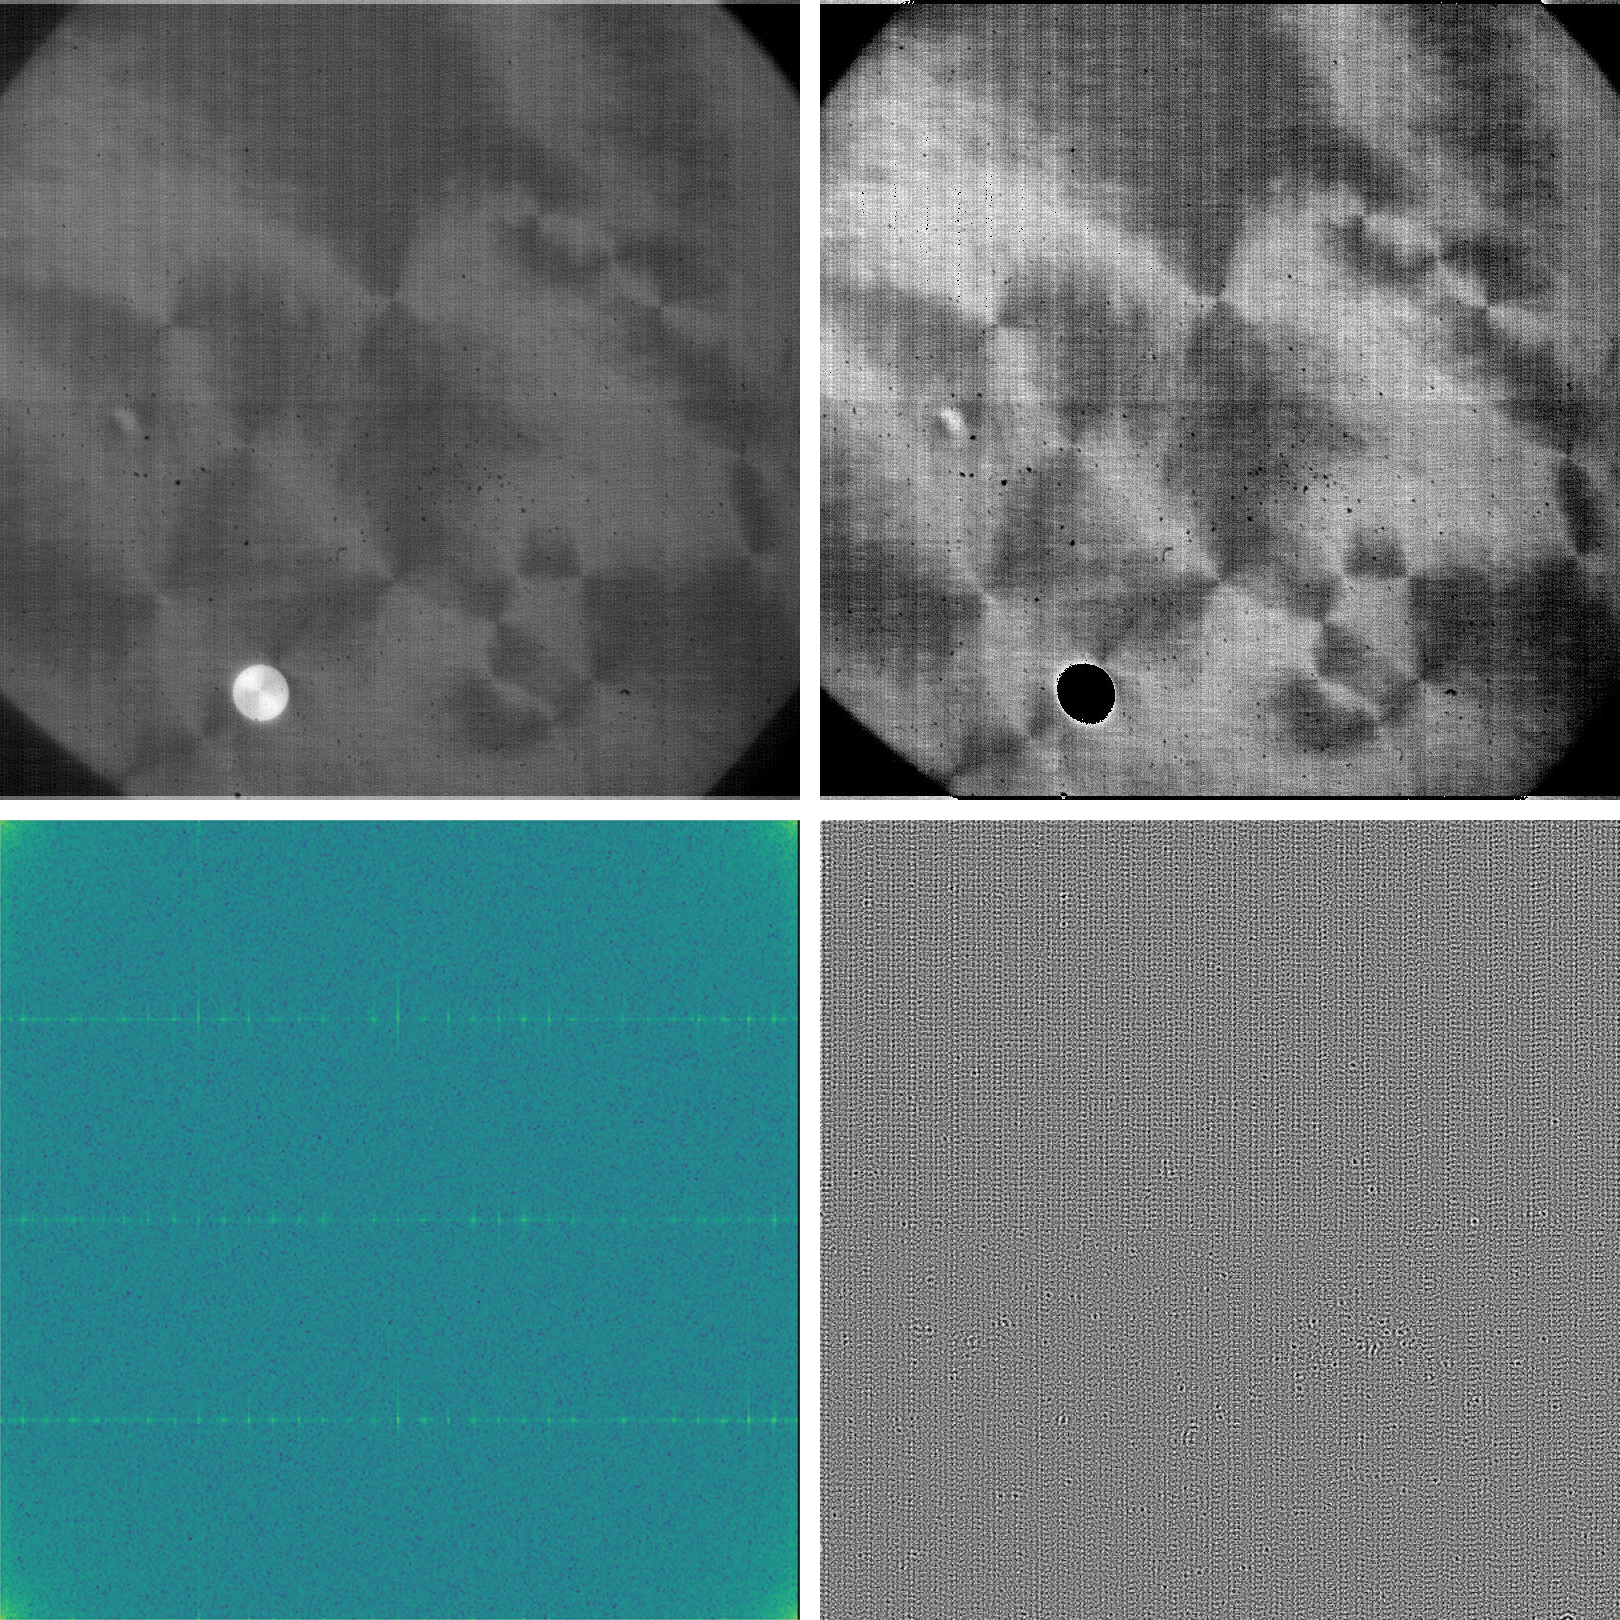
\includegraphics[width=\linewidth]{Standardizationandnoise.png}
  \caption{Image standardization and periodic noise extraction. Top-Left: Raw image. Top-Right: Standardized image. Bottom-Left: Fourier transform of standardized image. Bottom-Right: Noise extracted from the image.}
  \label{fig:Standardization and Noise}
\end{figure}

To further improve the simulation images, randomized Gaussian blurring is used to emulate the non-perfect and variable focus of the experimental data. Additionally, the overall brightness and dynamic range of the simulated images is randomized to prevent the model from being dependant on specific intensities or gradient magnitudes unique to the simulation.

FIGURE WITH GAUSSIAN BLURRING AND RANDOMIZED LIGHTING

The final components added to the simulated images were randomized lighting domains and circular artifacts. Observing the pattern of defect detections from previous models, it was discovered that detections would be made along lines where the lighting abruptly shifts. The microscope aperture and the boundaries between CCD sectors, which consistently read different pixel intensities, repeatedly generate such light shifts. (FIGURE SHOWING EXPERIMENTAL SECTOR CHANGES) To prevent this, the simulation images were broken into four quadrants of randomized size, with each quadrant having slightly different brightness. False detections would also be made around the boundaries of islands, which are circular objects present in liquid crystal films. To avoid this, circles of random brightness were added to the simulation data to provide negative counterexamples of non-defect objects that should be ignored.

FIGURE WITH NEGATIVE BOUNDARIES


\subsection{Effects of Simulated Image Enhancements}

In order to evaluate the effectiveness of each component in the pipeline, several models were trained on simulated images enhanced by the individual pipeline components and their efficacy evaluated. The models were validated using a hand annotated set of experimental images in order to determine how well they performed on real data.

Simulated images enhanced only by blurring, random islands and lighting quadrants, and randomized brightness and contrast produced models that were not viable for usage on experimental images. When validated, these models received recall scores of $<5\%$. Simulated images enhanced only with noise extracted using the Fourier transform produced a viable model, however the recall only reached $60\%$ with a recall of $40\%$. 

Combining Fourier noise with the other types of noise in the pipeline produced improvements to the model.



This supports the viability of training YOLO object detection models based on simulated data for use on experimental data.



\section{Results and Discussion}
\blindtext{}




%\begin{figure}[H]
%\centering
%\includegraphics[keepaspectratio=true,width=\columnwidth]{fig1-jem.png}
%\caption{write figure caption here}
%\label{fig:labelfighere}
%\end{figure}
%
%\bibliographystyle{apsrev4-1}
%\bibliography{../bibfilenamewithout.bib} % this is .bib file



\end{document}




